\subsection{E-step versus sleep phase}
\label{sec:estep_sleep_compare}

In this subsection, we compare the posteriors obtained by optimizing the E-step objective~\eqref{eq:e_step} versus optimizing the sleep-phase objective~\eqref{eq:sleep_phase_summary}. 
We demonstrate on a toy example that there exist shallow optima in E-step objective. In this example, the sleep phase objective is able to avoid the shallow optima, and the posterior is concentrated on the correct number of stars. 

In this toy example, we simulate a $20\times20$ image, show in figure 




We test on simulated data, so the wake-phase (M-step) is not needed. 


First, in Figure~\ref{fig:optim_path}, we print the optimization path of the ELBO over multiple restarts.  

\begin{figure}[!ht]
    \centering
    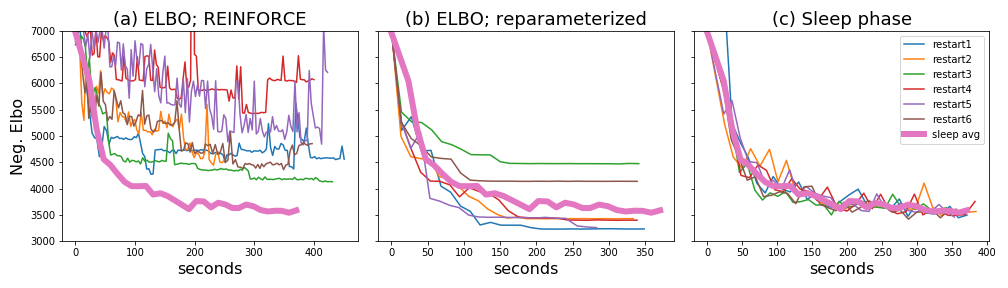
\includegraphics[width = \textwidth]{figures/optim_path_compare.png}
    \caption{ }
    \label{fig:optim_path}
\end{figure}
